\section{Dilution Conclusions}

The Dilution experiment allowed us to study the impact of flow on the collection of Coho eDNA samples. This study provided a  controlled environment to study the loss of eDNA signal via degradation  after the Coho had been removed from the tanks. The collection of plots organized in Table~\ref{fig:finalflowplot} illustrate the general trend. At the time of fish removal, TCT values were highest and sample replicates frequently had mean TCT values exceeding 15.  As seen in Figure~\ref{fig:finalflowplot}, at dilution levels of 160 kL and 1000 kL, TCT levels were not significantly different than background hatchery signals (Table~\ref{lab:flowzerofish}).

\vspace{5mm}

In the dilution experiment, Coho eDNA was detected at the 20kL dilution with 100\% reliability at the technical replicate level. At the 40kL level of dilution, Coho eDNA was detected in all but two sample replicates. Technical replicate non-detections occurred in eight of twelve sample. At 80kL dilution, only one sample replicate level detection was made, with 4 out of 8 qPCR replicates successfully amplifying target DNA. For dilutions greater than 80kL, we were not able to confirm presence with perfect detection, although several of the samples had 1 to 2 of 8 technical replicate detections.

\vspace{5mm}

We first fit several linear models, summarized in Table~\ref{lab:flowsum}.

\begin{table}[H]
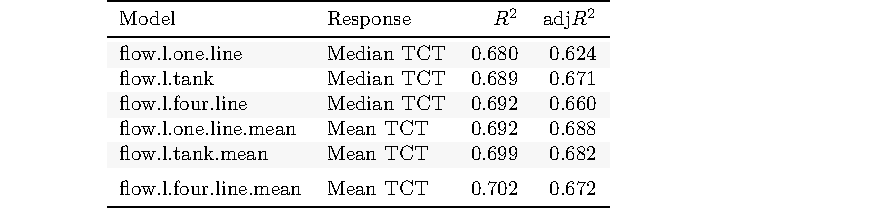
\includegraphics{Chapter4Images/flowsummary.pdf}
\caption{Table of comparison for the linear models fitted. Due to the breakpoint, we decided to leave linear models behind and work with non-linear models.}
\label{lab:flowsum}
\end{table}

\vspace{5mm}

Because there appeared to be a point at which the impact of dilution made Coho eDNA measurement negligible, we used a non-linear, bent cable model to fit a model for mean TCT. This model accounted for a  `break-point'. As seen in Figure~\ref{fig:bentcablemean}. Our breakpoint of $\log2(x)=6.89$ would represent a dilution of 118 kL. This could be thought of as the point at which Coho eDNA collection is no longer differentiable from the hatchery background signal. The confidence region for the breakpoint was computed by using the standard error of the model. The 95 \% confidence interval for the breakpoint ranged from 5.83 to 7.96 on the log2 scale. These points cover the range of dilutions from 56.96 kL to 247.28 kL. 